% Déclaration du type de document (report, book, paper, etc...)
\documentclass[a4paper]{paper} 
 
% Package pour avoir Latex en français
\usepackage[utf8]{inputenc}
\usepackage[T1]{fontenc}
 
% Quelques packages utiles
\usepackage{listings} % Pour afficher des listings de programmes
\usepackage{graphicx} % Pour afficher des figures
\usepackage{amsthm}   % Pour créer des théorèmes et des définitions
\usepackage{amsmath}
\usepackage{microtype} % Optical margins FTW
\usepackage{url}
\usepackage{booktabs} % Allows the use of \toprule, \midrule and \bottomrule in tables for horizontal lines
\usepackage{siunitx}
\usepackage{floatrow}
\usepackage{caption}
\usepackage{subcaption}
\usepackage{mhchem}
\usepackage[acronym,smallcaps]{glossaries}


% Début du document
\begin{document}
\begin{titlepage}

\newcommand{\HRule}{\rule{\linewidth}{0.5mm}} % Defines a new command for the horizontal lines, change thickness here

\center % Center everything on the page 
%----------------------------------------------------------------------------------------
%	HEADING 
%----------------------------------------------------------------------------------------
\textsc{\LARGE Club Vaudois de Robotique Autonome}\\[1.5cm] 

%----------------------------------------------------------------------------------------
%	TITLE 
%----------------------------------------------------------------------------------------
\HRule \\[0.4cm]
{ \huge \bfseries Eurobot 2014 : Pilot Study}\\[0.4cm] % Title of your document
\HRule \\[1.5cm]
 
%----------------------------------------------------------------------------------------
% LOGO EPFL
%----------------------------------------------------------------------------------------
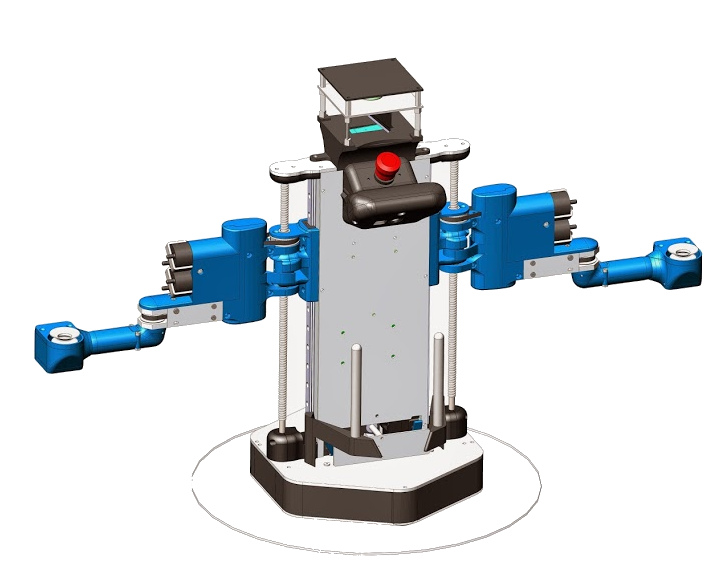
\includegraphics[width=\textwidth]{images/Debra_IV_1}\\[2cm] 

%----------------------------------------------------------------------------------------
%	AUTHORS 
%----------------------------------------------------------------------------------------

\vfill % Fill the rest of the page with whitespace

{\large \today}
\end{titlepage}




\section{General information}
\begin{itemize}
    \item This project study can be published before the contest.
    \item Team name : CVRA (Club Vaudois de Robotique Autonome).
    \item Team location : Renens, Switzerland.
    \item Budget : About 3000 \textsc{chf}, plus sponsors.
\end{itemize}

\section{Robots}
This year the club will engage two robots which are evolutions of previous years' designs.
The first one will have two arms, a differential drive and has code name \textit{Debra 5}.
The small robot isn't very advanced yet and is temporary named \textit{Nastya 3}.

\subsection{Debra 5}
\begin{figure}[h]
    \begin{center}
        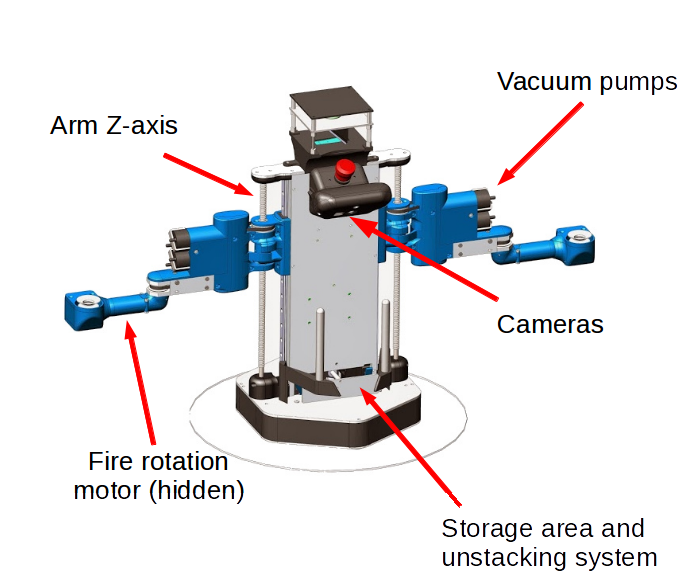
\includegraphics[width=0.6\textwidth]{images/debra_explained}
        \caption{Debra 5 robot.
            Height : \SI{350}{\milli\meter}.
            Perimeter : \SI{695}{\milli\meter}.
            Max perimeter is enforced by software.
        }
        \label{fig:debra}
    \end{center}
\end{figure}
Debra 5 is our big robot, dedicated to \textbf{todo}.

\paragraph{Motors}
Debra 5 uses two Faulhaber 2232-012-SR motors with a 20:1 reduction, rated at \SI{8.7}{\watt} at \SI{12}{\volt}, overvolted at \SI{14.8}{\volt}.
Those motors allows us to use our max acceleration (wheel slippage) to \SI{0.8}{\meter\per\second}.
All the motors in the robots are driven using custom power electronics.

\paragraph{Positioning}
Debra 5 will use a standard, encoder-based odometry to find its position on the table.

\paragraph{Opponent detection}
Our robots have two different avoidance system.
The first one is based on a rotating laser placed on opponent beacons, which allows to have absolute positionning.
The second one is based on a reflex sensor embedded in our robot which detects a reflector on the opponent system.
The redundancy allows for emergency stop in case of failure of the first one or of the pathfinding algorithm.

\begin{figure}[h]
    \begin{center}
        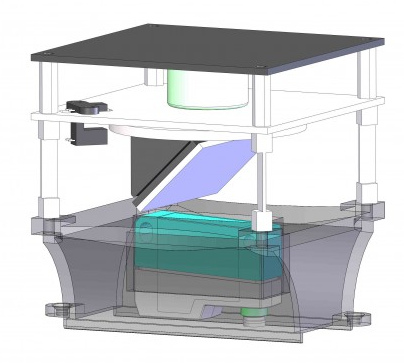
\includegraphics[width=0.6\textwidth]{images/Balise}
        \caption{Fallback beacon system.
            A reflex-type industrial sensor is mounted in the base (blue).
            It emits a LED beam (not laser), which is reflected on the rotating mirror (purple).
            A reflector is placed on the opponent robot, which allows for reliable detection.
            An index sensor (upper left, black) allows the robot to know the relative angle to opponent.
        }
        \label{fig:balise}
    \end{center}
\end{figure}

\paragraph{Power supply}
The robot is powered by a single \SI{14.8}{\volt} lithium-polymer battery, which gives us a run time of at least \SI{40}{\minute}.

\paragraph{Computing}
\begin{figure}[h]
    \begin{center}
        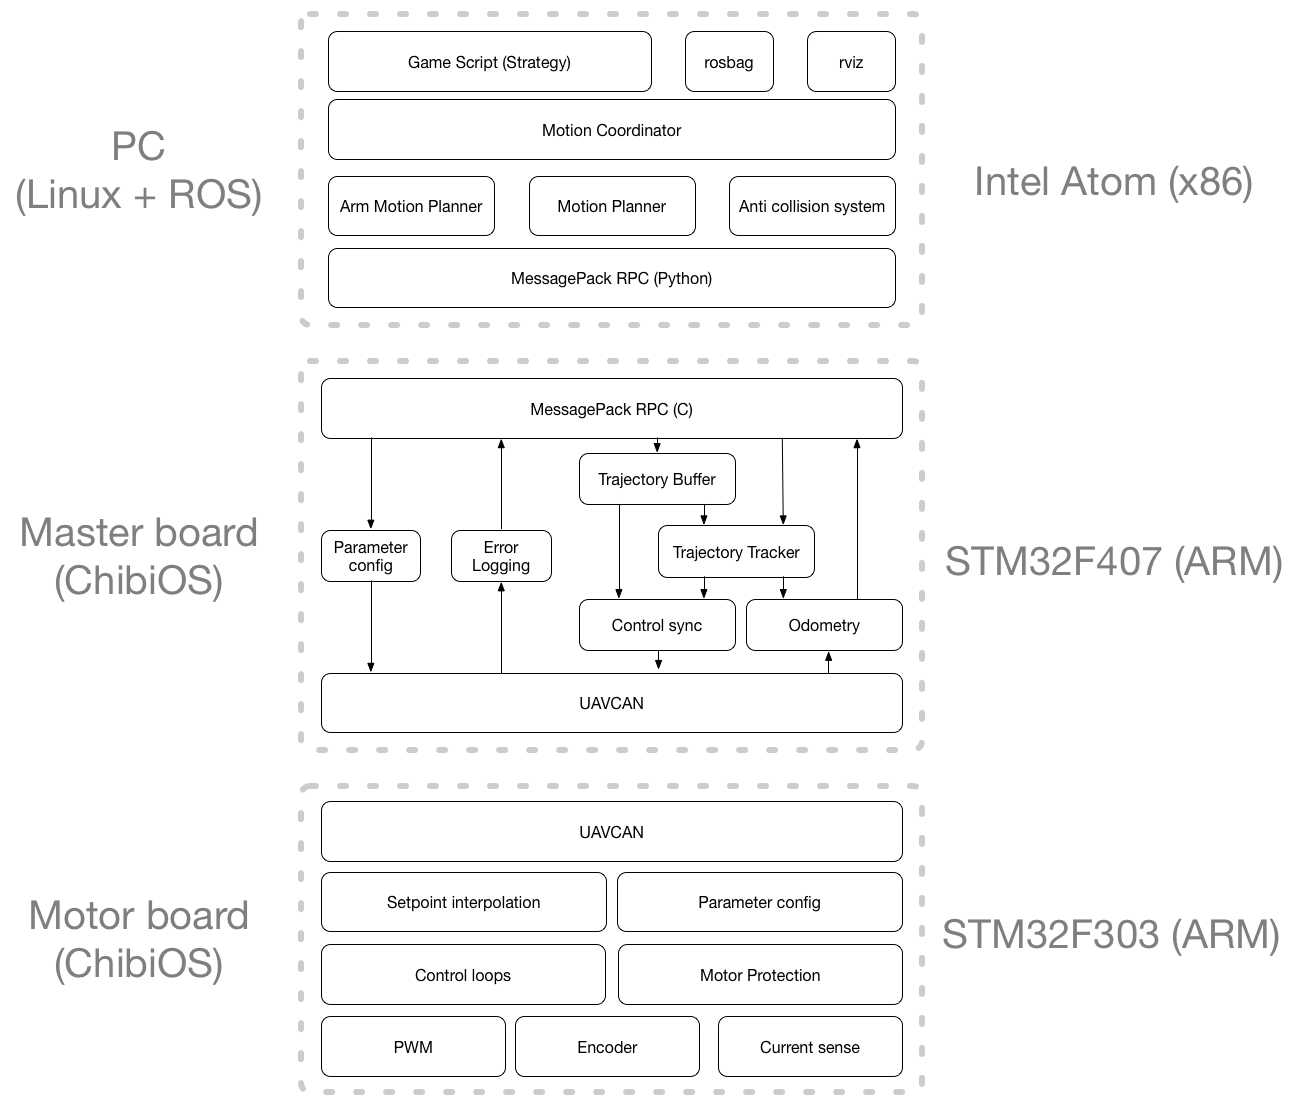
\includegraphics[width=0.6\textwidth]{images/software}
        \caption{Software architecture of our robot.}
        \label{fig:balise}
    \end{center}
\end{figure}

We have three different layers of computing in this year architecture (fig. \ref{fig:software}):
\begin{enumerate}
    \item An x86-based embedded PC running Linux is used for game decisisons and path planning.
    \item The realtime control is done on an ARM board which communicates with the PC using an IP/Ethernet link.
    \item Finally each motor has a motor control board connected to it, which is responsible for speed and torque control, motor protection etc.
        Communication with the main board is done via a CAN bus running at \si{1}{\mega\hertz}.
\end{enumerate}


This software architecture allows us to easily scale to any number of actuators or sensors in one robot (up to 127 motors per CAN bus/master board).

\subsection{Nastya 3}
Nastya's design is not finished yet, but most parts are common to both robots.

\section{Team members}
\begin{itemize}
    \item Antoine Albertelli, 21: Software engineer.
    \item Florian Reinhard, 21:  Software engineer.
    \item Patrick Spieler, 22:  Software engineer.
    \item Michael Spieler, 21:  Software engineer.
    \item Pius von Däniken, 23:  Software engineer.
    \item Romain Bersier, 29:  Mechanical engineer, Debra.
    \item Boris Pillionnel, 23:  Mechanical engineer, Nastya.
    \item Guillaume Schaufelberger, 19: Mechanical engineer, Nastya.
    \item Mathieu Rouvinez, 29:  Machining
    \item Jessica Schmid, 20: Electrical engineer.
    \item Dominik Reukauf, 24 : Mechanical Engineer.
\end{itemize}

\clearpage


\section{Sponsors}
\begin{figure}[h!]
    \centering
    \begin{subfigure}[h]{0.15\textheight}
        
\includegraphics[width=\textwidth]{images/sponsors/altera}
    \end{subfigure}%
    \hspace{1cm}
    \begin{subfigure}[h]{0.15\textheight}
        
\includegraphics[width=\textwidth]{images/sponsors/arrow}
    \end{subfigure}
    \vspace{0.4cm}


\vspace{0.4cm}


    \begin{subfigure}[h]{0.15\textheight}
        
\includegraphics[width=\textwidth]{images/sponsors/bossard}
    \end{subfigure}%
    \hspace{1cm}
    \begin{subfigure}[h]{0.15\textheight}
        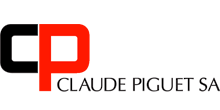
\includegraphics[width=\textwidth]{images/sponsors/claudePiguet}
    \end{subfigure}
\vspace{0.4cm}


    \begin{subfigure}[h]{0.15\textheight}
        
\includegraphics[width=\textwidth]{images/sponsors/faulhaber}
    \end{subfigure}%
    \hspace{1cm}
    \begin{subfigure}[h]{0.15\textheight}
        
\includegraphics[width=\textwidth]{images/sponsors/festo}
    \end{subfigure}
\vspace{0.4cm}


    \begin{subfigure}[h]{0.15\textheight}
        
\includegraphics[width=\textwidth]{images/sponsors/gardnerDenverThomas}
    \end{subfigure}%
    \hspace{1cm}
    \begin{subfigure}[h] {0.15\textheight}
        
\includegraphics[width=\textwidth]{images/sponsors/jauslin}
    \end{subfigure}
\vspace{0.4cm}


    \begin{subfigure}[h]{0.15\textheight}
        
\includegraphics[width=\textwidth]{images/sponsors/omron}
    \end{subfigure}%
    \hspace{1cm}
    \begin{subfigure}[h]{0.15\textheight}
        
\includegraphics[width=\textwidth]{images/sponsors/phoenixContact}
    \end{subfigure}
\vspace{0.4cm}


    \begin{subfigure}[h]{0.15\textheight}

        
\includegraphics[width=\textwidth]{images/sponsors/skf}
    \end{subfigure}%
    \hspace{1cm}
    \begin{subfigure}[h]{0.15\textheight}
        
\includegraphics[width=\textwidth]{images/sponsors/posic}
    \end{subfigure}
\vspace{0.4cm}


    \begin{subfigure}[h]{0.15\textheight}
        
\includegraphics[width=\textwidth]{images/sponsors/renens}
    \end{subfigure}%
    \hspace{1cm}
    \begin{subfigure}[h]{0.15\textheight}
        
\includegraphics[width=\textwidth]{images/sponsors/sick}
    \end{subfigure}
\vspace{0.4cm}


    \begin{subfigure}[h]{0.15\textheight}
        
\includegraphics[width=\textwidth]{images/sponsors/pmd}
    \end{subfigure}%
    \hspace{1cm}
    \begin{subfigure}[h]{0.15\textheight}
        
\includegraphics[width=\textwidth]{images/sponsors/SwissCNCTechnologies}
    \end{subfigure}
\vspace{0.4cm}


    \begin{subfigure}[h]{0.15\textheight}
        
\includegraphics[width=\textwidth]{images/sponsors/SwissMeo}
    \end{subfigure}%
    \hspace{1cm}
    \begin{subfigure}[h]{0.15\textheight}
        
\includegraphics[width=\textwidth]{images/sponsors/techniquesLaser}
    \end{subfigure}
\vspace{0.4cm}


\end{figure}


\end{document}
